
At a high level, LAVA adds bugs to programs in the following manner. For some specific input, we:

\begin {enumerate}
\item Identify execution trace locations where input bytes are available that do not determine control flow and have not been modified much. 
We call these quantities DUAs, for \underline{D}ead, \underline{U}ncomplicated and \underline{A}vailable data.
%We map these bytes back to their locations in the source code, and we later use this information to locate injection opportunities.
\item Find potential attack points that are temporally after a DUA in the program trace.
Attack points are source code locations where a DUA might be used, if only it were available there as well, to make a program vulnerable. 
\item Add code to the program to make the DUA value available at the attack point and use it to trigger the vulnerability. 
\end{enumerate}

These three steps will be discussed in the following three sections, which refer to the running example in Figure~\ref{fig:worked-example}.

\begin{figure}
\lstinputlisting[language=C,numbers=left, numberstyle=\tiny, stepnumber=2, numbersep=5pt,
        basicstyle=\ttfamily\footnotesize]{worked_example.c}
\caption{LAVA running example.  
Entering the function \texttt{foo}, \texttt{a} is bytes 0..3 of input, \texttt{b} is 4..7, and \texttt{n} is 8..11.
The pointers \texttt{s} and \texttt{d}, and the buffers pointed to by them are untainted.}
\label{fig:worked-example}
\end{figure}

\subsection {The DUA}

In a little more detail, the first step, in which DUAs are identified, is accomplished as follows.  

The program is executed under a dynamic taint analysis for a specific input.
\todo[inline]{Ricky: this is the first place we mention taint.  should we define our approach to taint analysis, maybe cite the papers that introduce the taint concepts we employ in LAVA?}
That taint analysis has a few important features.

\begin{itemize}
\item Each byte in the input is given its own label.
Thus, if an internal program quantity is tainted and is a direct copy of input bytes, then we can map that quantity back to a specific part of the input.
\item The taint analysis is as complete and correct as possible.  
All program code including library and kernel is subject to taint analysis.
Multiple threads and processes are also handled correctly, so that taint flows are not lost.
% operates, effectively, upon an LLVM-lifted version of the machine code for a program, including its libraries.
%This means taint is propagated accurately and completely, even through esoteric x86 instruction set extensions like MMX and SSE.
\item The taint analysis keeps track of a \emph{set} of labels per byte of program data, meaning that it can represent computation that mixes input bytes.
\end{itemize}
% We use the PANDA system to perform this taint analysis, with two crucial conceptual extensions in the form of taint-based measures.

\begin{figure}
\centering
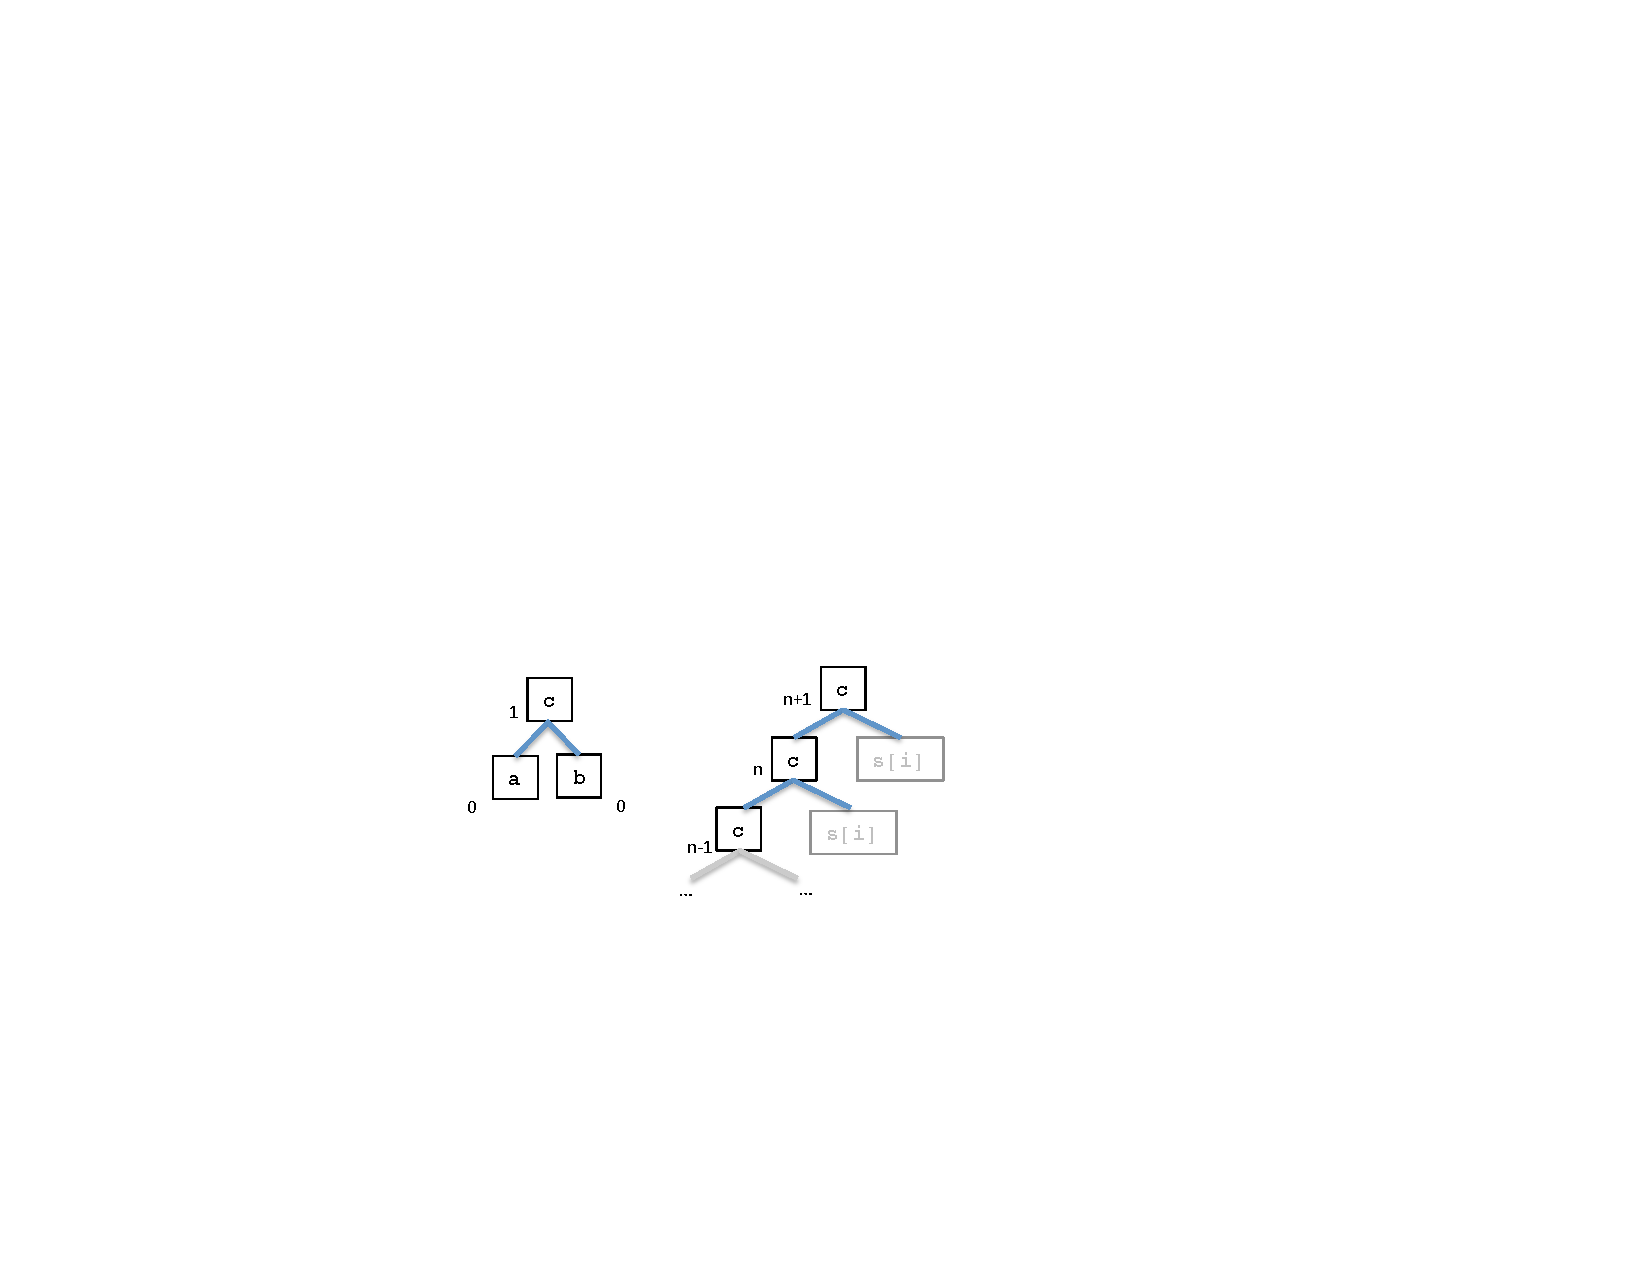
\includegraphics[width=3in]{tcn.pdf}
\caption{Taint Compute Number examples from the running example.  
TCN is simply the depth of the tree of computation that produces the value from tainted inputs.
TCN(c) after line 2 is 1, and after line 6 (upon exiting the loop), it is n+1.}
\label{fig:taint-compute-number}
\end{figure}

\noindent
Every tainted program variable is some function of the input bytes.
We estimate how complicated this function is via a new measure, the Taint Compute Number (TCN).
TCN simply tracks the depth of the tree of computation required to obtain a quantity from input bytes.
%TCN is illustrated in Figure~\ref{fig:taint-compute-number}; it simply tracks the depth of the tree of computation required to obtain 
%a quantity from input bytes.
The smaller TCN is for a program quantity, the closer it is, computationally, to the input.
If TCN is 0, the quantity is a direct copy of input bytes.
The intuition behind this measure is that we need DUAs that are computationally close to the input in order to be able to use them with predictable results.
Note that TCN is not an ideal measure.
There are obviously situations in which the tree of computation is deep but the resulting value is both completely predictable and has as much entropy as the original value.
However, TCN has the advantage that it is easy to compute on an instruction-by-instruction basis.
Whenever the taint system needs to union sets of taint labels to represent computation, the TCN associated with the resulting set is one more than the max of those of the 
input sets.
In the running example, and illustrated in Figure~\ref{fig:taint-compute-number}, $TCN(c)=1$ after line 1, since it is computed from quantities \verb+a+ and \verb+b+ which are directly derived from input.
Later, just before line 7 and after the loop, $TCN(c)=n+1$ because each iteration of the loop increases the depth of the tree of computation by one.  

The other taint-based measure LAVA introduces is \emph{Liveness}, which is associated with taint labels, i.e., the input bytes themselves.
This is a straightforward accounting of how many branches a byte in the input has been used to decide.
Thus, if a particular input byte label was never found in a taint label set associated with any byte used to decide a branch, it will have liveness of 0.
A DUA entirely consisting of bytes with 0 or very low liveness can be considered \emph{dead} in the sense that it can have little influence upon control flow for this program trace.
If one were to fuzz dead input bytes, the program should be indifferent and execute the same trace.  
In the running example, $LIV(0..3)=1$ after line 3, since \verb+a+ is a direct copy of input bytes 0..3.
After each iteration of the loop, the liveness of bytes 8..11, the loop bound, increase by one and so, after the loop, $LIV(8..11)=n$.

The combination of uncomplicated (low TCN) and dead (low liveness) program data is a powerful one for vulnerability injection.
The DUAs it identifies are internal program quantities that are often a direct copy of input bytes, and can be set to any chosen value without sending the program along a different path.  
These make very good triggers for vulnerabilities.
In the running example, bytes 0..3 and 8..11 are all somewhat live, because they have been seen to be used to decide branches.
Arguments \verb+a+ and \verb+n+ are therefore too live to be useful in injecting a vulnerability.
% XXX is this correct?  Is our example a bad one?
Argument \verb+b+, on the other hand, has a TCN of 0 and the bytes from which it derives, 4..7 are completely dead, 
making it an ideal trigger to control a vulnerability. 

Precisely which DUAs should be included, based on their liveness and TCN, is a configurable threshold. We explore the impact (in terms of whether the bug can be successfully injected and verified) of various thresholds in Section~\ref{sec:results:subsec:injection}.

\subsection {The attack point}

Attack point selection is a function of the type of vulnerability to be injected.
All that is required is that it must be possible to inject a bug at the attack point by making use of dead data.
This data can be made available later in the trace via new dataflow.
Obviously, this means that the attack point must be \emph{temporally after} an appearance of a DUA in the trace.
If the goal is to inject a read overflow, then reads via pointer dereference, array index, and bulk memory copy, e.g., are reasonable attack points.  
If the goal is to inject divide-by-zero, then arithmetic operations involving division will be attacked. 
Alternately, the goal might be to control one or more arguments to a library function.
For instance, in the running example, on line 7, the call to \verb+memcpy+ can be attacked since it is observed in the trace after a useable DUA, the argument \verb+b+, and any of its arguments can be controlled by adding \verb+b+, thus potentially triggering a buffer overflow. 

\subsection {Data-flow bug injection}

The third and final step to LAVA bug injection is introducing a dataflow relationship between DUA and attack point.  
If the DUA is in scope at the attack point then it can simply be used at the attack point to cause the vulnerability.
If it is not in scope, new code is added to siphon the DUA off into a safe place (perhaps in a static or global data structure), and later retrieve and make use of it at the attack point. 
However, in order to ensure that the bug only manifests itself very occasionally (one of our requirements from Section~\ref{sec:motivation}), we add a guard requiring that the DUA match a specific value if it is to be used to manifest the vulnerability.
In the running example, the DUA \verb+b+ is still in scope at the \verb+memcpy+ attack point and the only source code modification necessary is to make use of it to introduce the vulnerability if it matches a particular value.  
If we replace the first argument to the call to \verb+memcpy+, \verb+d+, with \verb-d+(b==0x6c617661)*b- then there will be an out of bounds write only when bytes 4..7 of the input exactly match 0x6c617661. 
